\section{Esplorazione dataset}\label{EsplorazioneDataset}
Il dataset oggetto di studio in questo progetto è relativo ad una partizione di prodotti di Amazon e dalle rispettive recensioni rilasciate dagli utenti. Esso è composto dalle due tabelle \textit{product} e \textit{reviews} descritte nel seguito sezioni \ref{Prodotti} e \ref{Recensioni}. I testi presenti in entrambe le tabelle sono in lingua italiana.

\subsection{Prodotti}\label{Prodotti}
La tabella \textit{product} è quella su cui si baserà l'analisi di rete e si compone dei seguenti campi:
\begin{itemize}
    \item \textbf{\_id}: codice alfanumerico identificativo del prodotto
    \item \textbf{title}: titolo del prodotto; rappresenta già di per sé una breve descrizione delle sue caratteristiche
    \item \textbf{category}: categoria di appartenenza del prodotto
    \item \textbf{price}: prezzo del prodotto in euro
    \item \textbf{avg\_rating}: media delle stelle delle recensioni sul prodotto; valore nell'intervallo [1.0, 5.0] 
    \item \textbf{reviews\_number}: numero totale di recensioni ricevute dal prodotto
    \item \textbf{questions\_number}: numero totale di domande poste dagli utenti sul prodotto
    \item \textbf{pictures}: url delle immagini relative al prodotto
    \item \textbf{description}: descrizione dettagliata del prodotto
    \item \textbf{features}: caratteristiche del prodotto
    \item \textbf{versions}: lista degli identificativi dei prodotti che rappresentano altre versioni dello stesso
    \item \textbf{bought\_together}: lista degli identificativi dei prodotti che vengono più spesso acquistati con il prodotto in questione nello stesso ordine; rappresenta una relazione tra prodotti
    \item \textbf{also\_bought}: lista degli identificativi dei prodotti che vengono più spesso acquistati in combinazione con il prodotto in questione; non necessariamente l'acquisto avviene nello stesso ordine; rappresenta una relazione tra prodotti
    \item \textbf{also\_viewed}: lista degli identificativi dei prodotti che vengono spesso più visualizzati da chi visualizza il prodotto in questione; rappresenta una relazione tra prodotti
\end{itemize}
Questa tabella raccoglie un totale di 20,459 prodotti, i quali si dividono in 37 categorie. La distribuzione nelle categorie è mostrata in figura \ref{fig:distribuzioneCategorie} e si può notare come essa sia particolarmente sbilanciata. \\
Le relazioni \textit{bought\_together}, \textit{also\_bought} e \textit{also\_viewed} che legano i prodotti sono fondamentali per effettuare un'analisi di rete e saranno approfondite nella sezione \ref{ReteProdotti}. Riguardo a queste relazioni è bene far notare che molti degli identificativi fanno riferimento a prodotti ignoti in quanto non compaiono nel dataset disponibile.

\begin{figure}[H]
    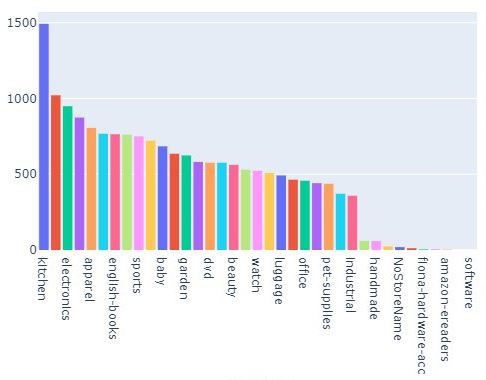
\includegraphics[scale=0.7]{distribuzioneCategorie}\centering
    \caption{Distribuzione dei prodotti tra le categorie}\label{fig:distribuzioneCategorie}
\end{figure}

\subsection{Recensioni}\label{Recensioni}
La tabella \textit{reviews}, che sarà oggetto di una sentiment analysis, si compone dei seguenti campi:
\begin{itemize}
    \item \textbf{\_id}: codice alfanumerico identificativo della recensione
    \item \textbf{product}: codice alfanumerico identificativo del prodotto a cui si riferisce la recensione
    \item \textbf{title}: titolo della recensione
    \item \textbf{author-id}: codice alfanumerico identificativo dell'autore della recensione
    \item \textbf{author-name}: nome dell'autore della recensione
    \item \textbf{date}: data in cui è stata scritta la recensione
    \item \textbf{rating}: voto in stelle dato al prodotto in questione; valore intero nell'intervallo [1, 5]
    \item \textbf{helpful}: numero di volte in cui la recensione è stata segnalata come utile da altri utenti
    \item \textbf{verified}: flag che rappresenta se la recensione sia relativa ad un acquisto verificato
    \item \textbf{body}: testo della recensione
\end{itemize} 
La tabella raccoglie un totale di 1,988,854 recensioni. In figura \ref{fig:distribuzioneRatingRecensioni} è possibile osservare una distribuzione fortemente sbilanciata verso le valutazioni positive, per questo motivo sarà importante bilanciare i dati nella fase di sentiment analysis. Come verrà mostrato alla sezione \ref{SentimentAnalysis}, gli attributi \textit{helpful} e \textit{verified} assumeranno un ruolo importante nel filtraggio del numero di recensioni. L'attributo \textit{body} costituirà invece il testo oggetto dell'analisi.\\
Nelle figure \ref{fig:wordCloudPos} e \ref{fig:wordCloudNeg} sono riportati rispettivamente i termini più frequenti per le recensioni positive (\textit{rating $>$ 3}) e negative (\textit{rating $<$ 3}). 
\begin{figure}[H]
    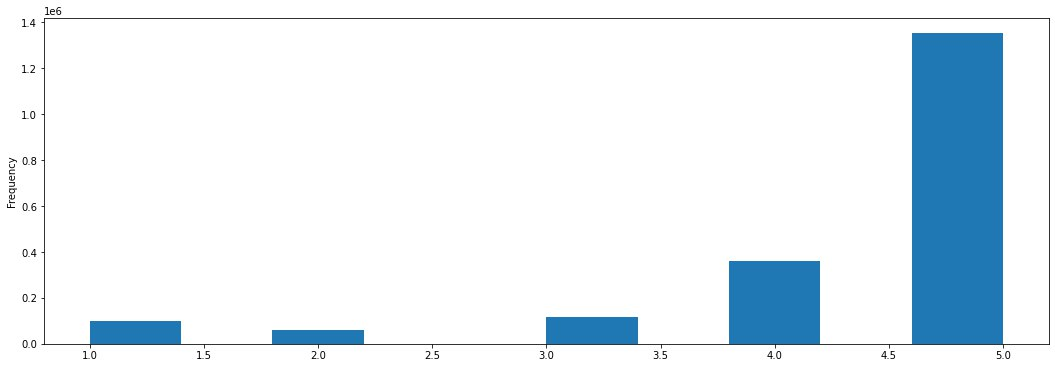
\includegraphics[scale=0.3]{distribuzioneRatingRecensioni}\centering
    \caption{Distribuzione del numero di stelle delle recensioni}\label{fig:distribuzioneRatingRecensioni}
\end{figure}
\begin{figure}[H]
    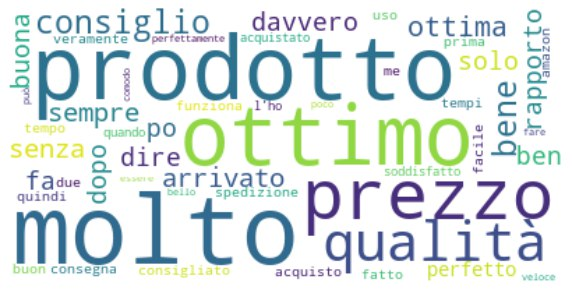
\includegraphics[scale=0.45]{wordCloudPos}\centering
    \caption{Word cloud delle parole che compaiono nelle recensioni positive}\label{fig:wordCloudPos}
\end{figure}
\begin{figure}[H]
    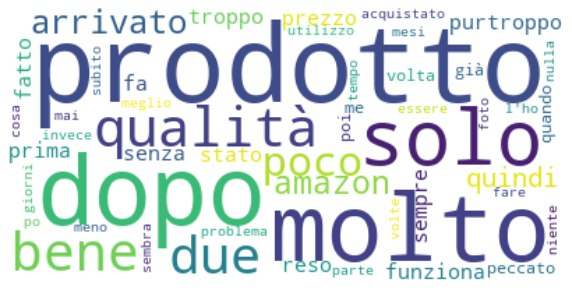
\includegraphics[scale=0.45]{wordCloudNeg}\centering
    \caption{Word cloud delle parole che compaiono nelle recensioni negative}\label{fig:wordCloudNeg}
\end{figure}



